\chapter{Resultados e Discussão}
\label{resultados-discussao}

Este capítulo descreve os testes realizados em relação ao sistema e a discussão sobre cada um deles.

\section{Método de teste}
\label{metodo-teste}
Os testes realizados tiveram como principal objetivo verificar a precisão e exatidão do GSMART em relação a
medição do tráfego de pessoas.

Os experimentos consistiram em deixar o sensor detectando dentro de zonas
selecionadas durante certos períodos de tempo (escolha aleatória e de acordo com a disponibilidade
dos donos). Buscou-se variar os ambientes de
detecção nos quesitos: concentração de pessoas e tempo de detecção. Para algumas
áreas menos concentradas foi possível registrar presencialmente o número de
pessoas por hora para comparação com os resultados do sistema. Em nenhum momento durante os experimentos
houve queda de energia, que impediria o escaneamento da zona.

Os métodos de avaliação estão centrados nos conceitos de: valor referência, média amostral e desvio padrão.
A variável quantitativa discreta identificada é o número de pessoas. O tratamento estatística adotado nos testes
é a inferência estatística (amostras) que é uma maneira rápida e econômica de fazer
inferência acerda da população \cite{Cabral2004}. As escolha do método de amostras
foi escolhido considerando que nem todos as horas foram monitoradas e as diferentes condições de
cada ambiente de teste.

\section{Terminologias estatísticas}
Antes de expor os testes e seus resultados é necessária uma revisão acerca de termos estatísticos segundo \citeonline{Cabral2004}. Eles são:
\begin{itemize}
    \item \textbf{valor verdadeiro}: o valor que obteríamos numa medição ideal, feita de condições
    perfeitas com instrumentos perfeitos e por operadores perfeitos;
    \item \textbf{exatidão:} a maior ou menor aproximação entre o resultado e o valor verdadeiro;
    \item \textbf{precisão:} está associada à dispersão dos valores resultantes da repetição das medições.
\end{itemize}

\section{Ambientes de teste}
Os ambientes de teste foram escolhidos de acordo com a disponibilidade de horário e autorização
para detecção. A condição que variou em cada um deles foi: concentração de pessoas e horários de detecção.
Outras características que influenciaram na detecção seram discutidos na \autoref{erros-influencia}.

\subsection{HOMEC}

Os testes nesta zona foram realizados em um edifício residencial com 4
andares, logo a antena capturou mais indivíduos do que os que se localizavam na área do apartamento (de  5 a 3 pessoas) durante as medições. As capturas foram coletadas numa sexta, entre
as 18:00 e as 23:00 horas, executadas de hora em hora dentro desse intervalo.

\subsection{HOMEJ}
Os testes foram realizados em um edifício residencial pequeno, com 3
andares e 6 apartamentos - por esse motivo, o alcance da antena capturou mais
indivíduos do que os que se localizavam na área do apartamento (4 pessoas)
durante as medições. São mostradas aqui as capturas coletadas numa sexta, entre
00:00 e 04:00 horas, executadas de hora em hora dentro desse intervalo, e no
sábado, em 2 intervalos (também efetuando-se a captura de hora em hora): 12:00
às 17:00 horas e 20:00 às 22:00 horas.

\subsection{LTIA}
Os testes nesta zona foram realizados no Laboratório de Tecnologia de Informação Aplicada, localizado no campus da UNESP em Bauru/SP. Durante o período de captura, haviam de 15 a 18 pessoas circulando pela área.  Os testes ocorreram das 16:00 às 18:00 horas, executados de hora em hora dentro desse intervalo. Devido à grande quantidade de máquinas e dispositivos no laboratório, houve uma certa disparidade na contagem de indivíduos.

\subsection{Camflam}
Os testes ocorreram no estabelecimento comercial Camflam Lanches, localizado em Bauru/SP. Durante o período de captura, não era possível saber a quantidade real de pessoas que circularam pela lanchonete.  Os testes ocorreram das 18:00 às 22:00 horas, executados de hora em hora dentro desse intervalo.

\section{Teste de precisão}
Os testes de precisão calculam as métricas estatísticas Variância ($S^{2}$) e Coeficiente de Variação (CV) das amostras obtidas, através da média aritmética entre todos os valores de contagem (Xi) obtidos de hora em hora e do Desvio Padrão. Foram realizados para cada zona. O valor do CV, nos 4 casos, mostrou-se bastante aceitável, sendo um pouco mais elevado na zona Camflam, onde ocorria de fato grande variação de frequentadores e não era possível saber antecipadamente quantas pessoas iriam ao estabelecimento.

Os valores para o CV estão em decimal e indicam uma porcentagem.

\begin{table}[]
\centering
\caption{Teste de precisão para a zona LTIA}
\label{ltia}
\begin{tabular}{cc|c|c|}
\hline
\multicolumn{1}{|c|}{Data e Hora}    & Contagem (Xi)         & Xi - \overline{X}          & (Xi - \overline{X})^{2} \\ \hline
\multicolumn{1}{|c|}{24-11-17 20:00} & 76                    & -4,67            & 21,8089    \\ \hline
\multicolumn{1}{|c|}{24-11-17 21:00} & 97                    & 16,33            & 266,6689   \\ \hline
\multicolumn{1}{|c|}{24-11-17 22:00} & 69                    & -11,67           & 136,1889   \\ \hline
\multicolumn{1}{l}{}                 & \multicolumn{1}{l|}{} & $S^{2}$ = \sum \limits_{i=1}^n \frac{(Xi - \overline{X})^{2}}{n-1} & 212,33335  \\ \cline{3-4}
\multicolumn{1}{l}{}                 & \multicolumn{1}{l|}{} & CV               & 0,18       \\ \cline{3-4}
\end{tabular}
\end{table}

\begin{table}[]
\centering
\caption{Teste de precisão para a zona HOMEJ}
\label{homej}
\begin{tabular}{cc|c|c|}
\hline
\multicolumn{1}{|c|}{Data e Hora}    & Contagem (Xi)         & Xi - \overline{X}         & (Xi - \overline{X})^{2} \\ \hline
\multicolumn{1}{|c|}{24-11-17 20:00} & 7                     & -5               & 25         \\ \hline
\multicolumn{1}{|c|}{24-11-17 21:00} & 11                    & -1               & 1          \\ \hline
\multicolumn{1}{|c|}{24-11-17 22:00} & 8                     & -4               & 16          \\ \hline
\multicolumn{1}{|c|}{25-11-17 00:00} & 19                    & 7                & 49         \\ \hline
\multicolumn{1}{|c|}{25-11-17 01:00} & 7                     & -5               & 25         \\ \hline
\multicolumn{1}{|c|}{25-11-17 02:00} & 8                     & -4               & 16         \\ \hline
\multicolumn{1}{|c|}{25-11-17 03:00} & 5                     & -7               & 49         \\ \hline
\multicolumn{1}{|c|}{25-11-17 12:00} & 15                    & 3                & 9          \\ \hline
\multicolumn{1}{|c|}{25-11-17 13:00} & 19                    & 7                & 49         \\ \hline
\multicolumn{1}{|c|}{25-11-17 14:00} & 18                    & 6                & 36         \\ \hline
\multicolumn{1}{|c|}{25-11-17 15:00} & 11                    & -1               & 1          \\ \hline
\multicolumn{1}{|l|}{25-11-17 16:00} & 16                    & 4                & 16         \\ \hline
\multicolumn{1}{|l|}{25-11-17 17:00} & 12                    & 0                & 0          \\ \hline
\multicolumn{1}{l}{}                 & \multicolumn{1}{l|}{} & $S^{2}$ = \sum \limits_{i=1}^n \frac{(Xi - \overline{X})^{2}}{n-1} & 24,33      \\ \cline{3-4}
\multicolumn{1}{l}{}                 & \multicolumn{1}{l|}{} & CV               & 0,411       \\ \cline{3-4}\end{tabular}
\end{table}

\begin{table}[]
\centering
\caption{Teste de precisão para a zona Camflam}
\label{camflam}
\begin{tabular}{cc|c|c|}
\hline
\multicolumn{1}{|c|}{Data e Hora}    & Contagem (Xi) & Xi - \overline{X}          & (Xi - \overline{X})^{2} \\ \hline
\multicolumn{1}{|c|}{25-11-17 18:00} & 179           & -72,4            & 5241,76    \\ \hline
\multicolumn{1}{|c|}{25-11-17 19:00} & 111           & -140,4           & 19712,16   \\ \hline
\multicolumn{1}{|c|}{25-11-17 20:00} & 115           & -136,4           & 18604,96   \\ \hline
\multicolumn{1}{|c|}{25-11-17 21:00} & 373           & 121,6            & 14786,56   \\ \hline
\multicolumn{1}{|c|}{25-11-17 22:00} & 479           & 227,6            & 51801,76   \\ \hline
                                     &               & $S^{2}$ = \sum \limits_{i=1}^n \frac{(Xi - \overline{X})^{2}}{n-1} & 27536,08   \\ \cline{3-4}
                                     &               & CV               & 0,66    \\ \cline{3-4}
\end{tabular}
\end{table}

\begin{table}[]
\centering
\caption{Teste de precisão para a zona HOMEC}
\label{homec}
\begin{tabular}{cc|c|c|}
\hline
\multicolumn{1}{|c|}{Data e Hora}    & Contagem (Xi) & Xi - \overline{X}          & (Xi - \overline{X})^{2} \\ \hline
\multicolumn{1}{|c|}{24-11-17 20:00} & 41            & 5                & 25         \\ \hline
\multicolumn{1}{|c|}{24-11-17 21:00} & 45            & 9                & 81         \\ \hline
\multicolumn{1}{|c|}{24-11-17 22:00} & 30            & -6               & 36         \\ \hline
\multicolumn{1}{|c|}{24-11-17 23:00} & 28            & -8               & 64         \\ \hline
                                     &               & $S^{2}$ = \sum \limits_{i=1}^n \frac{(Xi - \overline{X})^{2}}{n-1} & 68,67      \\ \cline{3-4}
                                     &               & CV               & 0,23      \\ \cline{3-4}
\end{tabular}
\end{table}


\section{Teste de exatidão}
\label{exatidao-teste}
O teste de exatidão compreende em dividir a média dos valores obtidos com GSMART
pela média dos valores reais. Desta operação, a resultante é a proporção do
número de dispositivos detectados pelo sistema em relação ao valores
verdadeiros. Quanto mais próximo de 1 for este resultado, mais acurado e exato
será o sensor.

Na \autoref{exato-ltia} sobre a zona LTIA, a média de valores encontrados pelo sensor foi 80,67,
enquanto a média real foi 15,67. Dividindo um valor pelo outro obtém-se 5,15. Portanto,
o sistema identificou 5,15 indivíduos e/ou dispositivos a mais do que o valor real.

\begin{table}[h]
\def\arraystretch{1.5}
\centering
\caption{Teste Exatidão para zona LTIA}
\label{exato-ltia}
\begin{tabular}{cccl}
\cline{1-3}
\multicolumn{1}{|c|}{\textbf{Data}}                                            & \multicolumn{1}{c|}{\textbf{Contagem GSMART}} & \multicolumn{1}{c|}{\textbf{Contagem Real}} &  \\ \cline{1-3}
\multicolumn{1}{|c|}{\begin{tabular}[c]{@{}c@{}}24-11-17\\ 16:00\end{tabular}} & \multicolumn{1}{c|}{76}                       & \multicolumn{1}{c|}{18}                     &  \\ \cline{1-3}
\multicolumn{1}{|c|}{\begin{tabular}[c]{@{}c@{}}24-11-17\\ 17:00\end{tabular}} & \multicolumn{1}{c|}{97}                       & \multicolumn{1}{c|}{15}                     &  \\ \cline{1-3}
\multicolumn{1}{|c|}{\begin{tabular}[c]{@{}c@{}}24-11-17\\ 18:00\end{tabular}} & \multicolumn{1}{c|}{69}                       & \multicolumn{1}{c|}{14}                     &  \\ \cline{1-3}
\overline{X}                                                                              & 80,67                                           & 15,67                                        &
\end{tabular}
\end{table}

Quando o teste é realizado para a zona HOMEC apresentado na \autoref{exato-homec}, a proporção encontrada é de 9 (36/4), demonstrando sendo ainda maior
que o valor encontrado anteriormente.
\begin{table}[h]
\def\arraystretch{1.5}
\centering
\caption{Teste Exatidão para zona HOMEC}
\label{exato-homec}
\begin{tabular}{cccl}
\cline{1-3}
\multicolumn{1}{|c|}{\textbf{Data}}                                            & \multicolumn{1}{c|}{\textbf{Contagem GSMART}} & \multicolumn{1}{c|}{\textbf{Contagem Real}} &  \\ \cline{1-3}
\multicolumn{1}{|c|}{\begin{tabular}[c]{@{}c@{}}24-11-17\\ 20:00\end{tabular}} & \multicolumn{1}{c|}{41}                       & \multicolumn{1}{c|}{5}                      &  \\ \cline{1-3}
\multicolumn{1}{|c|}{\begin{tabular}[c]{@{}c@{}}24-11-17\\ 21:00\end{tabular}} & \multicolumn{1}{c|}{45}                       & \multicolumn{1}{c|}{5}                      &  \\ \cline{1-3}
\multicolumn{1}{|c|}{\begin{tabular}[c]{@{}c@{}}24-11-17\\ 22:00\end{tabular}} & \multicolumn{1}{c|}{30}                       & \multicolumn{1}{c|}{3}                      &  \\ \cline{1-3}
\multicolumn{1}{|c|}{\begin{tabular}[c]{@{}c@{}}24-11-17\\ 23:00\end{tabular}} & \multicolumn{1}{c|}{28}                       & \multicolumn{1}{c|}{3}                      &  \\ \cline{1-3}
\overline{X}                                                                         & 36                                            & 4                                        &
\end{tabular}
\end{table}

Por fim, para a zona HOMEJ (\autoref{exato-homej}), o valor encontrado no teste foi 3 (12/4).

\begin{table}[h]
\def\arraystretch{1.5}
\centering
\caption{Teste Exatidão para zona HOMEJ}
\label{exato-homej}
\begin{tabular}{cccl}
\cline{1-3}
\multicolumn{1}{|c|}{\textbf{Data}}                                            & \multicolumn{1}{c|}{\textbf{Contagem GSMART}} & \multicolumn{1}{c|}{\textbf{Contagem Real}} &  \\ \cline{1-3}
\multicolumn{1}{|c|}{\begin{tabular}[c]{@{}c@{}}24-11-17\\ 20:00\end{tabular}} & \multicolumn{1}{c|}{7}                        & \multicolumn{1}{c|}{4}                      &  \\ \cline{1-3}
\multicolumn{1}{|c|}{\begin{tabular}[c]{@{}c@{}}24-11-17\\ 21:00\end{tabular}} & \multicolumn{1}{c|}{11}                       & \multicolumn{1}{c|}{4}                      &  \\ \cline{1-3}
\multicolumn{1}{|c|}{\begin{tabular}[c]{@{}c@{}}24-11-17\\ 22:00\end{tabular}} & \multicolumn{1}{c|}{8}                        & \multicolumn{1}{c|}{4}                      &  \\ \cline{1-3}
\multicolumn{1}{|c|}{\begin{tabular}[c]{@{}c@{}}25-11-17\\ 00:00\end{tabular}} & \multicolumn{1}{c|}{19}                       & \multicolumn{1}{c|}{4}                      &  \\ \cline{1-3}
\multicolumn{1}{|c|}{\begin{tabular}[c]{@{}c@{}}25-11-17\\ 01:00\end{tabular}} & \multicolumn{1}{c|}{7}                        & \multicolumn{1}{c|}{4}                      &  \\ \cline{1-3}
\multicolumn{1}{|c|}{\begin{tabular}[c]{@{}c@{}}25-11-17\\ 02:00\end{tabular}} & \multicolumn{1}{c|}{8}                        & \multicolumn{1}{c|}{4}                      &  \\ \cline{1-3}
\multicolumn{1}{|c|}{\begin{tabular}[c]{@{}c@{}}25-11-17\\ 03:00\end{tabular}} & \multicolumn{1}{c|}{5}                        & \multicolumn{1}{c|}{4}                      &  \\ \cline{1-3}
\multicolumn{1}{|c|}{\begin{tabular}[c]{@{}c@{}}25-11-17\\ 12:00\end{tabular}} & \multicolumn{1}{c|}{15}                       & \multicolumn{1}{c|}{4}                      &  \\ \cline{1-3}
\multicolumn{1}{|c|}{\begin{tabular}[c]{@{}c@{}}25-11-17\\ 13:00\end{tabular}} & \multicolumn{1}{c|}{19}                       & \multicolumn{1}{c|}{4}                      &  \\ \cline{1-3}
\multicolumn{1}{|c|}{\begin{tabular}[c]{@{}c@{}}25-11-17\\ 14:00\end{tabular}} & \multicolumn{1}{c|}{18}                       & \multicolumn{1}{c|}{4}                      &  \\ \cline{1-3}
\multicolumn{1}{|c|}{\begin{tabular}[c]{@{}c@{}}25-11-17\\ 15:00\end{tabular}} & \multicolumn{1}{c|}{11}                       & \multicolumn{1}{c|}{4}                      &  \\ \cline{1-3}
\multicolumn{1}{|c|}{\begin{tabular}[c]{@{}c@{}}25-11-17\\ 16:00\end{tabular}} & \multicolumn{1}{c|}{16}                       & \multicolumn{1}{c|}{4}                      &  \\ \cline{1-3}
\multicolumn{1}{|c|}{\begin{tabular}[c]{@{}c@{}}25-11-17\\ 17:00\end{tabular}} & \multicolumn{1}{c|}{12}                       & \multicolumn{1}{c|}{4}                      &  \\ \cline{1-3}
\overline{X}                                                                   & 12                                            & 4                                           &
\end{tabular}
\end{table}

Esse teste não foi executado com a zona Camflam, pois não foi possível obter os valores reais da quantidade
de clientes.

\subsection{Avaliação exatidão}
O teste de exatidão mostra que nenhum dos valores encontrados das proporções da zonas em relação aos valores
verdadeiros é igual a 1 (ideal), expondo que o GSMART identifica mais dispositivos do que indíviduos dentro
de cada zona. Portanto, o GSMART não pode ser considera um sistema exato, pois distancia-se dos valores referência.


\section{Testes empíricos}
Depois de testes sobre exatidão e precisão que buscaram quantificar e expressar através de métricas
as conclusões, através da observação e discussão - empirismo - surgiram importantes temas a serem debatidos
a seguir.

\subsection{Análise da curva de crescimento dos gráficos}
Após realizar os testes é possível observar que o sistema não fornece informações
que expressem uma realidade quantitativa. Entretanto, através do método
empírico, nota-se que a curva de crescimento dos gráficos pode estimar o tráfego
de pessoas quanto aos pontos: se houve queda, quando houve horários de pico,
horários de menor movimento, entre outros. Por exemplo, ao confrontar a \autoref{homec-graph} que representa
o gráfico de detecção da zona HOMEC com os dados reais (veja \autoref{exatidao-teste}), percebe-se que
o sensor conseguiu detectar a variação de pessoas dentro do ambiente. Nesse caso, na duas primeiras horas havia 5 pessoas, na 2 horas
seguintes o gráfico decresce, confirmando o decaimento também do número de indíviduos que foi para 4.

\begin{figure}[!h]
  \caption{\label{homec-graph}Gráfico da zona HOMEC}
  \begin{center}
    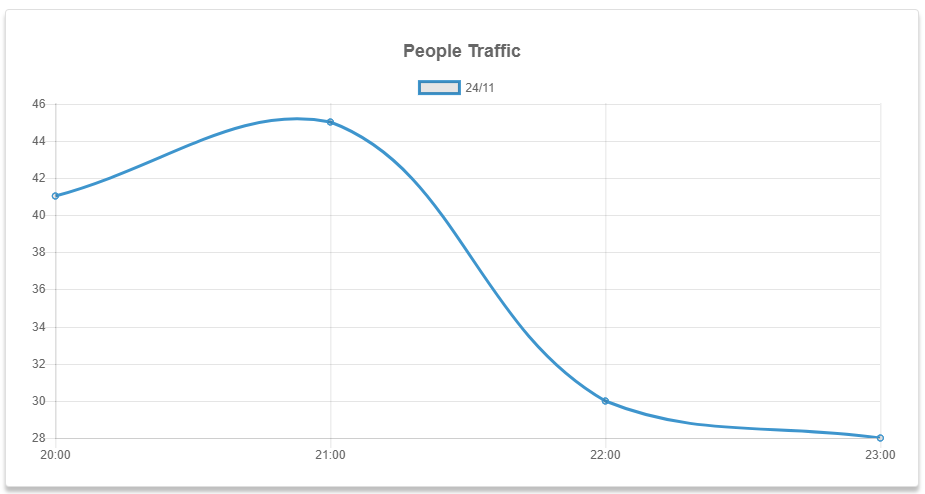
\includegraphics[width=0.90\textwidth]{img/graph-homec.png}
  \end{center}
  \legend{Fonte: Elaborada pelas autoras.}
\end{figure}

No gráfico da zona Camflam que está na \autoref{camflam-graph}, observa-se que
há crescimento relevante entre ás 20:00 e 22:00. Em conversa, com o proprietário
do restaurante e com os garçons foi confirmado, que o horário de pico ocorreu
entre as 21:30 e 22:30, mais uma vez corroborando para o cenário trazido por este
gráfico, onde o pico encontra-se às 22:00. O restaurante abre às 18:00, assim como visto,
na \autoref{camflam-graph} foi um do horários de baixo tráfego.


\begin{figure}[!h]
  \caption{\label{camflam-graph}Gráfico da zona Camflam}
  \begin{center}
    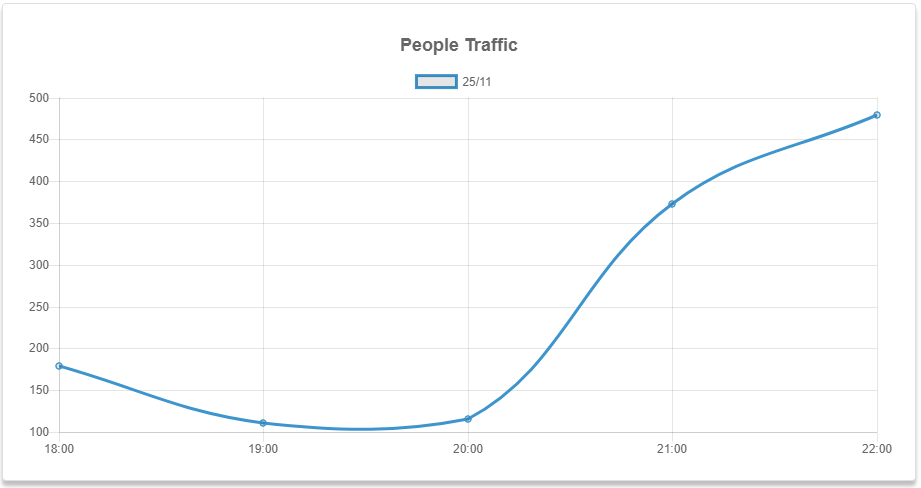
\includegraphics[width=0.90\textwidth]{img/camflam-graph.png}
  \end{center}
  \legend{Fonte: Elaborada pelas autoras.}
\end{figure}

\subsection{Informações propostas}
Na \autoref{diaria} descrevemos que informações foram derivadas dos dados capturados. Acerca delas e a partir
dos testes realizados descritos neste capítulo, é possíve inferir que a informação sobre o pico de tráfego
é a que melhor corresponde o comportamento real do tráfego. Apesar de não saber indicar o quanto realmente houve de pico, o
horário pode ser identificado, assim como discutimos na subseção anterior.

Sobre os fabricantes notou-se certa tendência em todas as zonas das fabricantes Samsung e Motorola estarem
sempre dentre as primeiras, observe os gráficos de setor na \autoref{graf1} e \autoref{graf2}. Não é possível afirmar se de fato corresponde a proporção real, pois o intervalo de envio
de \emph{probe requests} muda de acordo com o fabricante. Além disso, a Apple emprega técnicas que dificultam
a identificação da marca através do endereço MAC, a técnica utilizada é a randomização de MACs e verificações passivas \cite{Apple2016}.

\begin{figure}[!h]
  \caption{\label{graf1}Fabricantes encontrados na zona Camflam}
  \begin{center}
    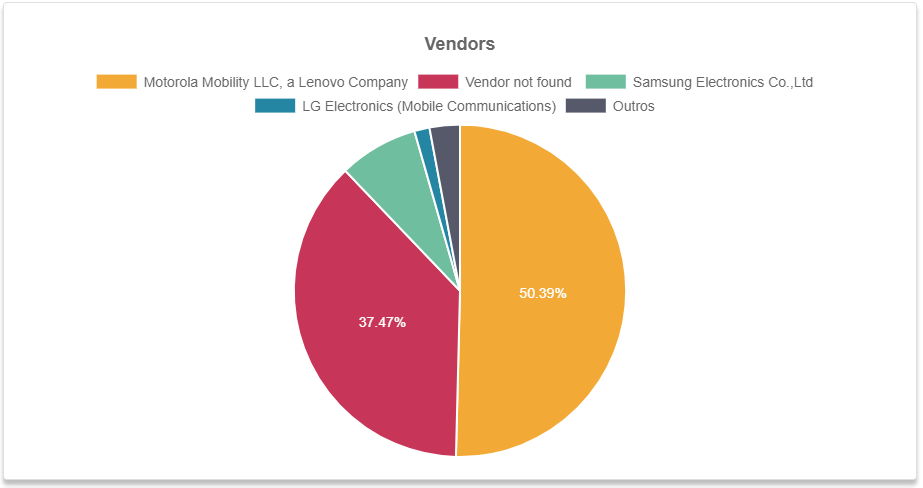
\includegraphics[width=0.90\textwidth]{img/setor-camflam.png}
  \end{center}
  \legend{Fonte: Elaborada pelas autoras.}
\end{figure}

\begin{figure}[!h]
  \caption{\label{graf2}Fabricantes encontrados na zona HOMEJ}
  \begin{center}
    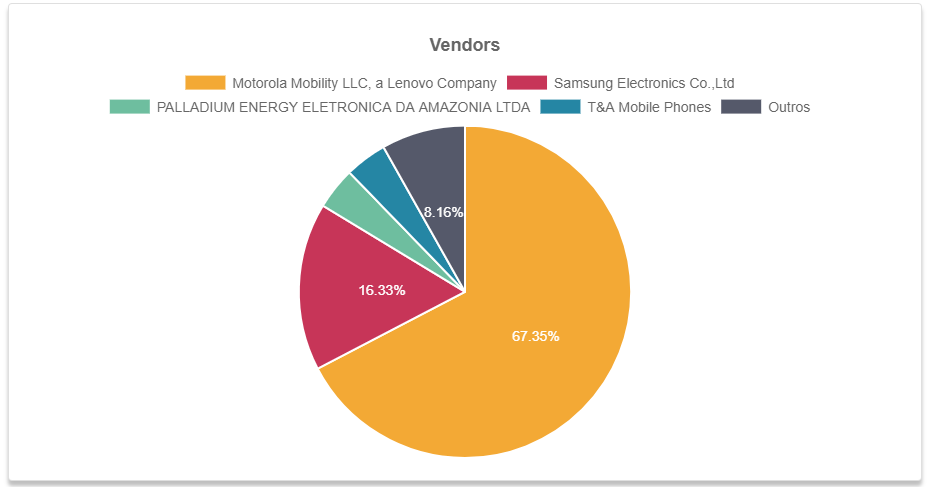
\includegraphics[width=0.90\textwidth]{img/setor.png}
  \end{center}
  \legend{Fonte: Elaborada pelas autoras.}
\end{figure}

\section{Erros e influenciadores na medição}
\label{erros-influencia}
Conclui-se a partir dos testes que o sistema proposto neste trabalho não é exato - não
representa os valores reais - e possui uma precisão de medição entre 18\% e
66\%. Além disso observou-se alguns pontos que podem ter levado às diferenças nas medições:
\begin{itemize}
    \item \textbf{Passagem rápida}: pessoas que passam rapidamente pelas zonas são contadas, mesmo que não
    permaneçam por muito tempo;
    \item \textbf{Dispositivos ao redor}: o número de dispositivos móveis ao redor da zona,como computadores, tablets,
    ou mais de um aparelho por pessoa, influenciam no aumento significativo no número de dispositivos identificados;
    \item \textbf{Antena Wi-Fi não ligada}: se o indíviduo não estive pelor menos com a antena Wi-Fi ligada, mesmo sem
    estar associado a nenhum AP, o sensor não o detecta;
    \item \textbf{Número de aparelhos por indíviduo}: se um indíviduo estiver portando mais de um aparelho
    móvel, será contabilizado duas vezes.
    \item \textbf{Zonas morta}: devido ao formato da onde de Wi-Fi, há zonas em que o sinal não consegue
    detectar ninguém, perdendo estes dispositivos na contagem.
\end{itemize}
